% Šablona pro maturitní práci Gymnázia Jírovcova 8, České Budějovice
% Autoři šablony: Jonáš Havelka, Michal Kočer, Daniel Sýkora
% Typ dokumentu: report
% veškeré úpravy v soubor MP.sty (styl maturitní práce)
\documentclass[12pt]{report}
% %%%%%%%%%%%%%%%%%%%%%%%%%%%%%%%%%%%%%%%%%%%%%%%%%%%%%%%
\usepackage{MP}						  % Import stylu maturitní práce
\author{Kryštof Maxera}                  % AUTOR PRÁCE
\title{Konstrukce dronu}    % NÁZEV PRÁCE
\date{14. února 2025}                 % DATUM ODEVZDÁNÍ PRÁCE
\vedouci{Dr.rer.nat Michal Kočer} % VEDOUCÍ PRÁCE
\place{V Českých Budějovicích}
\skolnirok{2024/2025}                  % ŠKOLNí ROK
\logo{
\includegraphics[scale=1.25]{GJ8_logotyp}} %Logo školy
%%%%%%%%%%%%%%%%%%%%%%%%%%%%%%%%%%%%%%%%%%%%%%%%%%%%%%%%%%%%%%%%%%%
\begin{document} %%%%%%% začátek dokumentu
%%%%%%%%%%%%%%%%%%%%%%%%%%%%  Titulní stránka + úvodní povinné stránky
\pagenumbering{roman}                   % číslování stránek římskými číslicemi
	\mytitlepage						% Vygenerování titulní strany
	
	\prohlaseni{
		Prohlašuji, že jsem tuto práci vypracoval samostatně s vyznačením všech použitých pramenů.
	}	
	
	\abstrakt{
		\lipsum[1]						% Abstrakt 
	}{
		\lipsum[1]						% Klíčová slova
	}
	
	\podekovani{
		\lipsum[2]						% Poděkování
	}
	
   {\tableofcontents\newpage}			% Obsah
	
%%%%%%%%%%%%%%%%%%%%%%%%%%%% VLASTNÍ PRÁCE
\addtocounter{page}{1}		% Posunutí countru stránek
\pagenumbering{arabic}		% Číslování stránek arabskými číslicemi
\chapter*{Úvod}     % úvod práce 
	
\lipsum[1]	
	
%%%%%%%%%%%%%% TEORETICKÁ ČÁST %%%%%%%%%%%%%%%%%%	
\part{Úvod do světa dronů}  % název teoretické části (nenechávejte Teoretická část)
	
\chapter{Definice a charakteristika dronů}
			
Dron je definován jako zařízení nebo stroj schopný vykonávat úkoly bez nutnosti přímé fyzické přítomnosti člověka. Tato zařízení lze rozdělit do dvou základních kategorií. \\
\\První kategorii tvoří plně autonomní roboti, u jichž je přítomnost člověka vyžadována primárně z kontrolních a bezpečnostních důvodu. Pilot nebo operátor zde většinou nezasahuje do aktivního řízení, ale v případě potřeby může převzít kontrolu. Typickým příkladem jsou autonomní bezpilotní letadla s možností vzdáleného ovládání nebo samořízené motorové vozidlo, které ke svému provozu nepotřebuje řidiče přítomného ve vozidle. \\
\\Druhá kategorie je pro veřejnost známější. Její součástí jsou dálkově ovládaná zařízení, která nejsou plně autonomní. Do této skupiny patří široce známé kvadrokoptéry a další multikoptéry, stejně jako autíčka na dálkové ovládání.\\
\\Důvodem časté záměny těchto dvou kategorií je překrývání některých funkcí, neboť i dálkově ovládané kvadrokoptéry využívají automatické systémy, například pro samovyvažování, které jsou nezbytné pro jejich stabilní let.\\
\\Drony lze obecně rozdělit do tří hlavních podskupin na základě prostředí, ve kterém operují:
\begin{itemize}
	\item \textbf{Bezpilotní letadla} - (UAVs - Unmanned Aerial Vehicles)
	\item \textbf{Dálkově ovládaná podvodní vozidla} - (ROUVs - Remotely Operated Underwater Vehicles)
	\item \textbf{Pozemní vozidla} - (Rovers)
\end{itemize}
V této práci se zaměříme na konstrukci kvadrokoptéry, která spadá do kategorie bezpilotních letadel. \cite{byod}\\


\section{Druhy dronů}
	Odkaz v závorkách: \parencite[see][page 900]{einstein}\\
	Odkaz: \cite{knuthwebsite}\\
	A odkaz pod čarou: \footcite[see][s. 42]{latexcompanion}\\
	Dobrý den, ahoj, \gls{atd}\\
	Praha, \gls{tj} hlavní město ČR
	
	\begin{table}
 		\caption{Testovací tabulka}
		\label{tab:test2}
			\begin{tabular}{ccccc}
				1 & 1 & 1  & 1  & 1  \\
				1 & 2 & 3  & 4  & 5  \\
				1 & 3 & 6  & 10 & 15 \\
				1 & 4 & 10 & 30 & 45
				\end{tabular}
	\end{table}

\lipsum[2]

\chapter[Stručná historie dronů]{Stručná historie dronů}
%%% v obsahu se objeví jen to co je v hranatých závorkách
\begin{figure}
  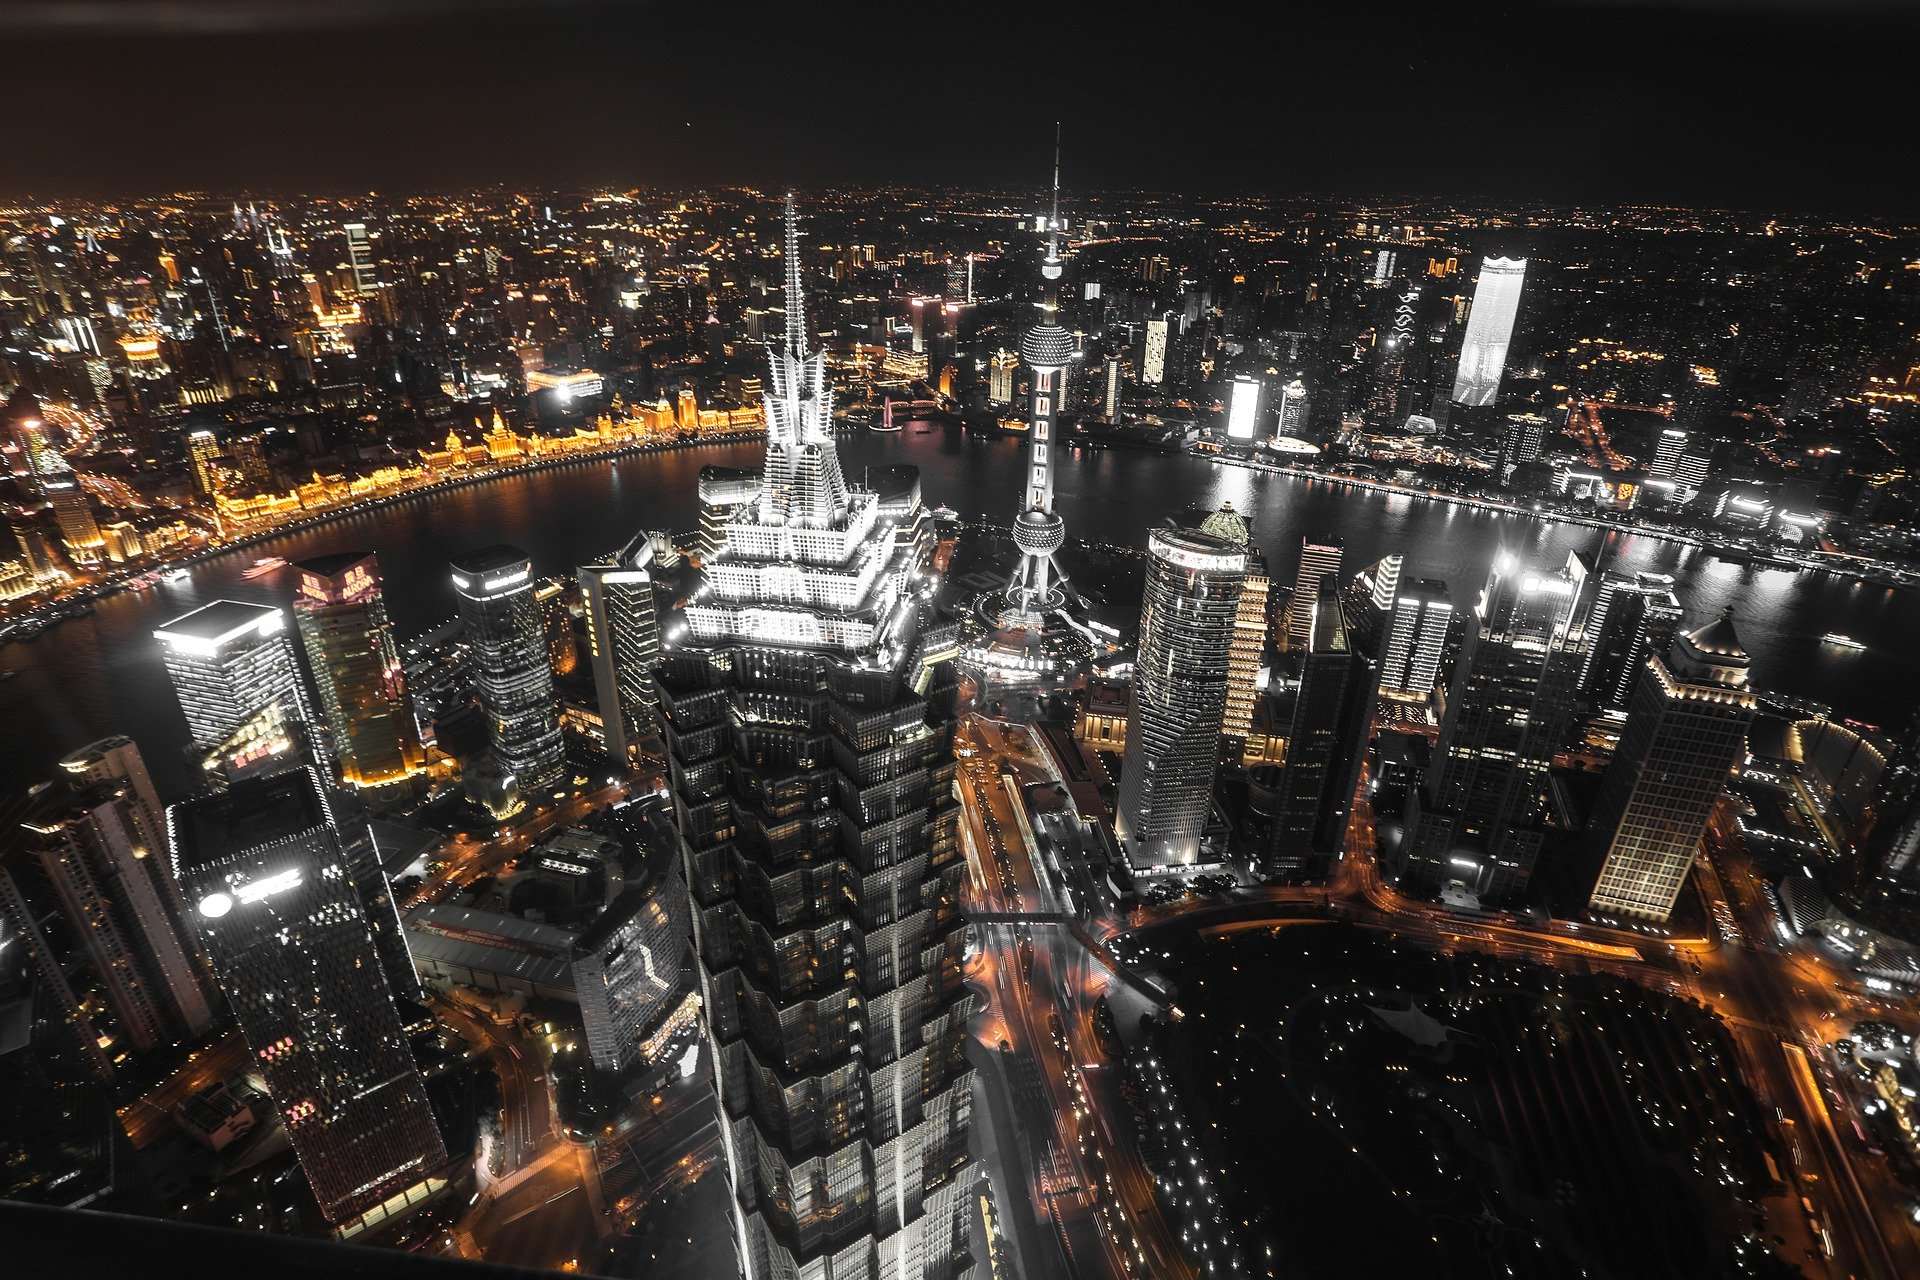
\includegraphics[width=\linewidth]{test.jpg}
  \caption{Testovací}
  \label{fig:test}
\end{figure}
Obrázek \ref{fig:test} ukazuje Shangai z Pixabay.\\
Tabulka \ref{tab:test2} ukazuje hádejte, co.
	
\lipsum[3]

\chapter{Anatomie dronu}
			
\section{Motory}

\lipsum[1]

\section{ESP}

\lipsum[2]

\section{Baterie}

\lipsum[3]

\section{Raspberry Pi Pico}

\lipsum[4]

\chapter{Fyzika letu dronu}

\lipsum[1]

%%%%%%%%%%%%%% PRAKTICKÁ ČÁST %%%%%%%%%%%%%%%%%%	
\part{Konstrukce kvadrokoptéry} % název praktické části (nenechávejte název Praktická část)

\chapter{Součástky}
\lipsum[1]	

\chapter{Průběh Konstrukce}

\lipsum[1]	

Výpis programu \nameref{lst:hello_world}  naleznete ve výpise \ref{lst:hello_world}.

\begin{lstlisting}[title={Program hello.c}, caption={hello.c}, label={lst:hello_world}]
#include <stdio.h>
#define CISLO 10

int main(void) {
	int i = CISLO;

	print("Hello World!\n");
	print("%d", i);

	return (0);
}
\end{lstlisting}

\lipsum[1]	

\begin{lstlisting}[numbers=none, title={Příklad výstupního souboru}]
11.0524
5.5954
6.7996
13.8584
15.1357
Soucet: 52.4415
\end{lstlisting}

\chapter{Program}

\lipsum[1]

\chapter{Schéma zapojení}

\lipsum[1]

%%%%%%%%%%%%% ZÁVĚR
\chapter*{Závěr}
	
\lipsum[1]
	
\nocite{*}
\printbibliography					% Vytvoří seznam literatury
\addcontentsline{toc}{chapter}{Bibliografie}
\printglossary[title={Zkratky}]		% Vytvoří seznam zkratek
\listoffigures						% Vytvoří seznam obrázků
\listoftables						% Vytvoří seznam tabulek

%%%%%%%%%%%%% PŘÍLOHY - APPENDIX 	
\begin{appendices}
	\chapter{Fotografie zkonstruované kvadrokoptéry}	
	\lipsum[1]
    	%\pitem{Fotky z pokusů}
    	%\eitem{Vlastní program}
    	%\eitem{Dokumentace}
    	%\eitem{Testovací data}
	\chapter{Kód programu Raspberry Pi Pico}  
\end{appendices}
%%%%%%%%%%%%%%%
\end{document}
%%%%%%%%%%%%%%%%%%%% KONEC %%%%%%%%%%%%%%%%%%%%%%%%%